\documentclass[tikz, border=10pt]{standalone}
\usepackage{pgfplots}
\pgfplotsset{compat=1.18}
\usepackage{siunitx}

\begin{document}
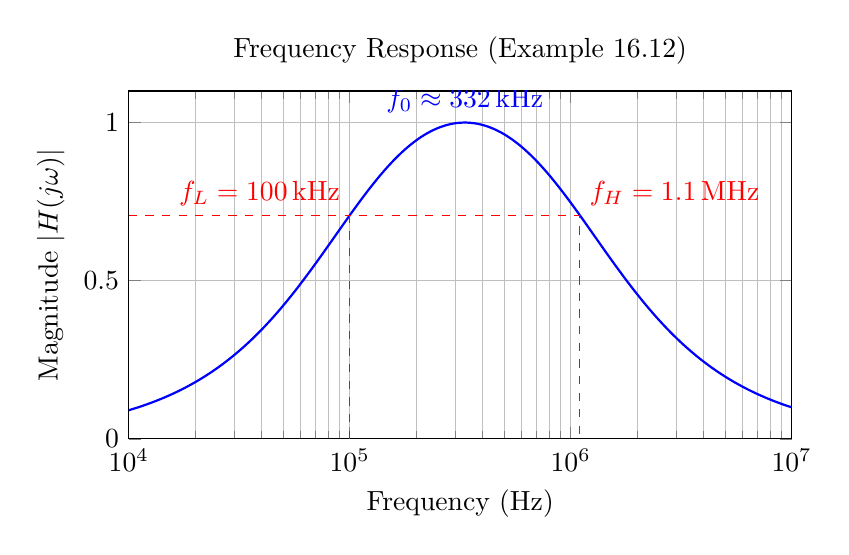
\begin{tikzpicture}
    \begin{semilogxaxis}[
        width=10cm, height=6cm,
        title={Frequency Response (Example 16.12)},
        xlabel={Frequency (Hz)},
        ylabel={Magnitude $|H(j\omega)|$},
        grid=both,
        xmin=1e4, xmax=1e7,
        ymin=0, ymax=1.1,
        samples=500,
        domain=1e4:1e7,
    ]
    
    % Parameters
    % R = 628.3
    % L = 100e-6
    % C = 2.3e-9
    % H(f) = (2*pi*f*R*C) / sqrt( (1 - (2*pi*f)^2 * L * C)^2 + (2*pi*f*R*C)^2 )
    
    \addplot[thick, blue, variable=\f] 
    { (2*pi*f*628.3*2.3e-9) / sqrt( (1 - (2*pi*f)^2 * 100e-6 * 2.3e-9)^2 + (2*pi*f*628.3*2.3e-9)^2 ) };
    
    % Mark Cutoff Frequencies
    % fL = 100 kHz = 1e5
    % fH = 1.1 MHz = 1.1e6
    \draw[dashed, red] (axis cs: 1e5, 0) -- (axis cs: 1e5, 0.707) -- (axis cs: 1.1e6, 0.707) -- (axis cs: 1.1e6, 0);
    \draw[dashed, red] (axis cs: 1e4, 0.707) -- (axis cs: 1e5, 0.707);
    
    \node[anchor=south east, red] at (axis cs: 1e5, 0.707) {$f_L = \SI{100}{kHz}$};
    \node[anchor=south west, red] at (axis cs: 1.1e6, 0.707) {$f_H = \SI{1.1}{MHz}$};
    \node[anchor=south, blue] at (axis cs: 3.317e5, 1) {$f_0 \approx \SI{332}{kHz}$};
    
    \end{semilogxaxis}
\end{tikzpicture}
\end{document}
